\documentclass[1p]{elsarticle_modified}
%\bibliographystyle{elsarticle-num}

%\usepackage[colorlinks]{hyperref}
%\usepackage{abbrmath_seonhwa} %\Abb, \Ascr, \Acal ,\Abf, \Afrak
\usepackage{amsfonts}
\usepackage{amssymb}
\usepackage{amsmath}
\usepackage{amsthm}
\usepackage{scalefnt}
\usepackage{amsbsy}
\usepackage{kotex}
\usepackage{caption}
\usepackage{subfig}
\usepackage{color}
\usepackage{graphicx}
\usepackage{xcolor} %% white, black, red, green, blue, cyan, magenta, yellow
\usepackage{float}
\usepackage{setspace}
\usepackage{hyperref}

\usepackage{tikz}
\usetikzlibrary{arrows}

\usepackage{multirow}
\usepackage{array} % fixed length table
\usepackage{hhline}

%%%%%%%%%%%%%%%%%%%%%
\makeatletter
\renewcommand*\env@matrix[1][\arraystretch]{%
	\edef\arraystretch{#1}%
	\hskip -\arraycolsep
	\let\@ifnextchar\new@ifnextchar
	\array{*\c@MaxMatrixCols c}}
\makeatother %https://tex.stackexchange.com/questions/14071/how-can-i-increase-the-line-spacing-in-a-matrix
%%%%%%%%%%%%%%%

\usepackage[normalem]{ulem}

\newcommand{\msout}[1]{\ifmmode\text{\sout{\ensuremath{#1}}}\else\sout{#1}\fi}
%SOURCE: \msout is \stkout macro in https://tex.stackexchange.com/questions/20609/strikeout-in-math-mode

\newcommand{\cancel}[1]{
	\ifmmode
	{\color{red}\msout{#1}}
	\else
	{\color{red}\sout{#1}}
	\fi
}

\newcommand{\add}[1]{
	{\color{blue}\uwave{#1}}
}

\newcommand{\replace}[2]{
	\ifmmode
	{\color{red}\msout{#1}}{\color{blue}\uwave{#2}}
	\else
	{\color{red}\sout{#1}}{\color{blue}\uwave{#2}}
	\fi
}

\newcommand{\Sol}{\mathcal{S}} %segment
\newcommand{\D}{D} %diagram
\newcommand{\A}{\mathcal{A}} %arc


%%%%%%%%%%%%%%%%%%%%%%%%%%%%%5 test

\def\sl{\operatorname{\textup{SL}}(2,\Cbb)}
\def\psl{\operatorname{\textup{PSL}}(2,\Cbb)}
\def\quan{\mkern 1mu \triangleright \mkern 1mu}

\theoremstyle{definition}
\newtheorem{thm}{Theorem}[section]
\newtheorem{prop}[thm]{Proposition}
\newtheorem{lem}[thm]{Lemma}
\newtheorem{ques}[thm]{Question}
\newtheorem{cor}[thm]{Corollary}
\newtheorem{defn}[thm]{Definition}
\newtheorem{exam}[thm]{Example}
\newtheorem{rmk}[thm]{Remark}
\newtheorem{alg}[thm]{Algorithm}

\newcommand{\I}{\sqrt{-1}}
\begin{document}

%\begin{frontmatter}
%
%\title{Boundary parabolic representations of knots up to 8 crossings}
%
%%% Group authors per affiliation:
%\author{Yunhi Cho} 
%\address{Department of Mathematics, University of Seoul, Seoul, Korea}
%\ead{yhcho@uos.ac.kr}
%
%
%\author{Seonhwa Kim} %\fnref{s_kim}}
%\address{Center for Geometry and Physics, Institute for Basic Science, Pohang, 37673, Korea}
%\ead{ryeona17@ibs.re.kr}
%
%\author{Hyuk Kim}
%\address{Department of Mathematical Sciences, Seoul National University, Seoul 08826, Korea}
%\ead{hyukkim@snu.ac.kr}
%
%\author{Seokbeom Yoon}
%\address{Department of Mathematical Sciences, Seoul National University, Seoul, 08826,  Korea}
%\ead{sbyoon15@snu.ac.kr}
%
%\begin{abstract}
%We find all boundary parabolic representation of knots up to 8 crossings.
%
%\end{abstract}
%\begin{keyword}
%    \MSC[2010] 57M25 
%\end{keyword}
%
%\end{frontmatter}

%\linenumbers
%\tableofcontents
%
\newcommand\colored[1]{\textcolor{white}{\rule[-0.35ex]{0.8em}{1.4ex}}\kern-0.8em\color{red} #1}%
%\newcommand\colored[1]{\textcolor{white}{ #1}\kern-2.17ex	\textcolor{white}{ #1}\kern-1.81ex	\textcolor{white}{ #1}\kern-2.15ex\color{red}#1	}

{\Large $\underline{12a_{0226}~(K12a_{0226})}$}

\setlength{\tabcolsep}{10pt}
\renewcommand{\arraystretch}{1.6}
\vspace{1cm}\begin{tabular}{m{100pt}>{\centering\arraybackslash}m{274pt}}
\multirow{5}{120pt}{
	\centering
	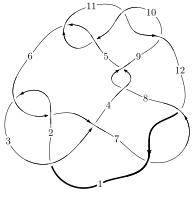
\includegraphics[width=112pt]{../../../GIT/diagram.site/Diagrams/png/1027_12a_0226.png}\\
\ \ \ A knot diagram\footnotemark}&
\allowdisplaybreaks
\textbf{Linearized knot diagam} \\
\cline{2-2}
 &
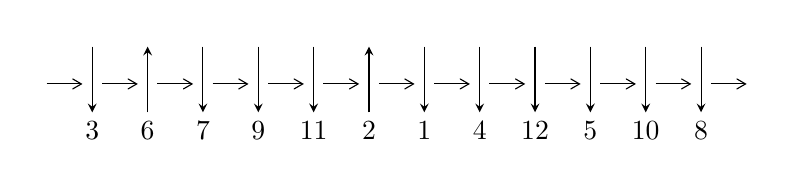
\begin{tikzpicture}[x=20pt, y=17pt]
	% nodes
	\node (C0) at (0, 0) {};
	\node (C1) at (1, 0) {};
	\node (C1U) at (1, +1) {};
	\node (C1D) at (1, -1) {3};

	\node (C2) at (2, 0) {};
	\node (C2U) at (2, +1) {};
	\node (C2D) at (2, -1) {6};

	\node (C3) at (3, 0) {};
	\node (C3U) at (3, +1) {};
	\node (C3D) at (3, -1) {7};

	\node (C4) at (4, 0) {};
	\node (C4U) at (4, +1) {};
	\node (C4D) at (4, -1) {9};

	\node (C5) at (5, 0) {};
	\node (C5U) at (5, +1) {};
	\node (C5D) at (5, -1) {11};

	\node (C6) at (6, 0) {};
	\node (C6U) at (6, +1) {};
	\node (C6D) at (6, -1) {2};

	\node (C7) at (7, 0) {};
	\node (C7U) at (7, +1) {};
	\node (C7D) at (7, -1) {1};

	\node (C8) at (8, 0) {};
	\node (C8U) at (8, +1) {};
	\node (C8D) at (8, -1) {4};

	\node (C9) at (9, 0) {};
	\node (C9U) at (9, +1) {};
	\node (C9D) at (9, -1) {12};

	\node (C10) at (10, 0) {};
	\node (C10U) at (10, +1) {};
	\node (C10D) at (10, -1) {5};

	\node (C11) at (11, 0) {};
	\node (C11U) at (11, +1) {};
	\node (C11D) at (11, -1) {10};

	\node (C12) at (12, 0) {};
	\node (C12U) at (12, +1) {};
	\node (C12D) at (12, -1) {8};
	\node (C13) at (13, 0) {};

	% arrows
	\draw[->,>={angle 60}]
	(C0) edge (C1) (C1) edge (C2) (C2) edge (C3) (C3) edge (C4) (C4) edge (C5) (C5) edge (C6) (C6) edge (C7) (C7) edge (C8) (C8) edge (C9) (C9) edge (C10) (C10) edge (C11) (C11) edge (C12) (C12) edge (C13) ;	\draw[->,>=stealth]
	(C1U) edge (C1D) (C2D) edge (C2U) (C3U) edge (C3D) (C4U) edge (C4D) (C5U) edge (C5D) (C6D) edge (C6U) (C7U) edge (C7D) (C8U) edge (C8D) (C9U) edge (C9D) (C10U) edge (C10D) (C11U) edge (C11D) (C12U) edge (C12D) ;
	\end{tikzpicture} \\
\hhline{~~} \\& 
\textbf{Solving Sequence} \\ \cline{2-2} 
 &
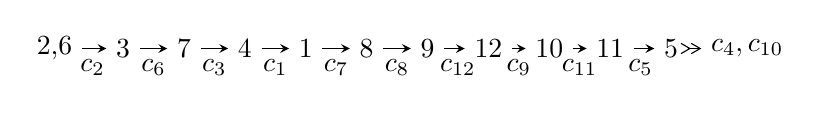
\begin{tikzpicture}[x=22pt, y=7pt]
	% node
	\node (A0) at (-1/8, 0) {2,6};
	\node (A1) at (1, 0) {3};
	\node (A2) at (2, 0) {7};
	\node (A3) at (3, 0) {4};
	\node (A4) at (4, 0) {1};
	\node (A5) at (5, 0) {8};
	\node (A6) at (6, 0) {9};
	\node (A7) at (7, 0) {12};
	\node (A8) at (8, 0) {10};
	\node (A9) at (9, 0) {11};
	\node (A10) at (10, 0) {5};
	\node (C1) at (1/2, -1) {$c_{2}$};
	\node (C2) at (3/2, -1) {$c_{6}$};
	\node (C3) at (5/2, -1) {$c_{3}$};
	\node (C4) at (7/2, -1) {$c_{1}$};
	\node (C5) at (9/2, -1) {$c_{7}$};
	\node (C6) at (11/2, -1) {$c_{8}$};
	\node (C7) at (13/2, -1) {$c_{12}$};
	\node (C8) at (15/2, -1) {$c_{9}$};
	\node (C9) at (17/2, -1) {$c_{11}$};
	\node (C10) at (19/2, -1) {$c_{5}$};
	\node (A11) at (45/4, 0) {$c_{4},c_{10}$};

	% edge
	\draw[->,>=stealth]	
	(A0) edge (A1) (A1) edge (A2) (A2) edge (A3) (A3) edge (A4) (A4) edge (A5) (A5) edge (A6) (A6) edge (A7) (A7) edge (A8) (A8) edge (A9) (A9) edge (A10) ;
	\draw[->>,>={angle 60}]	
	(A10) edge (A11);
\end{tikzpicture} \\ 

\end{tabular} \\

\footnotetext{
The image of knot diagram is generated by the software ``\textbf{Draw programme}" developed by Andrew Bartholomew(\url{http://www.layer8.co.uk/maths/draw/index.htm\#Running-draw}), where we modified some parts for our purpose(\url{https://github.com/CATsTAILs/LinksPainter}).
}\phantom \\ \newline 
\centering \textbf{Ideals for irreducible components\footnotemark of $X_{\text{par}}$} 
 
\begin{align*}
I^u_{1}&=\langle 
u^{90}+u^{89}+\cdots+u-1\rangle \\
\\
\end{align*}
\raggedright * 1 irreducible components of $\dim_{\mathbb{C}}=0$, with total 90 representations.\\
\footnotetext{All coefficients of polynomials are rational numbers. But the coefficients are sometimes approximated in decimal forms when there is not enough margin.}
\newpage
\renewcommand{\arraystretch}{1}
\centering \section*{I. $I^u_{1}= \langle u^{90}+u^{89}+\cdots+u-1 \rangle$}
\flushleft \textbf{(i) Arc colorings}\\
\begin{tabular}{m{7pt} m{180pt} m{7pt} m{180pt} }
\flushright $a_{2}=$&$\begin{pmatrix}1\\0\end{pmatrix}$ \\
\flushright $a_{6}=$&$\begin{pmatrix}0\\u\end{pmatrix}$ \\
\flushright $a_{3}=$&$\begin{pmatrix}1\\- u^2\end{pmatrix}$ \\
\flushright $a_{7}=$&$\begin{pmatrix}u\\u\end{pmatrix}$ \\
\flushright $a_{4}=$&$\begin{pmatrix}u^4+u^2+1\\u^4\end{pmatrix}$ \\
\flushright $a_{1}=$&$\begin{pmatrix}u^2+1\\- u^4\end{pmatrix}$ \\
\flushright $a_{8}=$&$\begin{pmatrix}- u^7-2 u^5-2 u^3\\u^9+u^7+u^5+u\end{pmatrix}$ \\
\flushright $a_{9}=$&$\begin{pmatrix}- u^{17}-4 u^{15}-9 u^{13}-12 u^{11}-11 u^9-8 u^7-6 u^5-4 u^3- u\\- u^{17}-3 u^{15}-5 u^{13}-4 u^{11}- u^9+u\end{pmatrix}$ \\
\flushright $a_{12}=$&$\begin{pmatrix}u^{12}+3 u^{10}+5 u^8+4 u^6+2 u^4+u^2+1\\- u^{14}-2 u^{12}-3 u^{10}-2 u^8-2 u^6-2 u^4- u^2\end{pmatrix}$ \\
\flushright $a_{10}=$&$\begin{pmatrix}u^{43}+10 u^{41}+\cdots-5 u^3-2 u\\- u^{45}-9 u^{43}+\cdots+u^3+u\end{pmatrix}$ \\
\flushright $a_{11}=$&$\begin{pmatrix}u^{74}+17 u^{72}+\cdots+3 u^2+1\\- u^{76}-16 u^{74}+\cdots-3 u^4-2 u^2\end{pmatrix}$ \\
\flushright $a_{5}=$&$\begin{pmatrix}- u^{30}-7 u^{28}+\cdots-4 u^4+1\\- u^{30}-6 u^{28}+\cdots+2 u^4+u^2\end{pmatrix}$\\&\end{tabular}
\flushleft \textbf{(ii) Obstruction class $= -1$}\\~\\
\flushleft \textbf{(iii) Cusp Shapes $= -4 u^{89}-4 u^{88}+\cdots+4 u-10$}\\~\\
\newpage\renewcommand{\arraystretch}{1}
\flushleft \textbf{(iv) u-Polynomials at the component}\newline \\
\begin{tabular}{m{50pt}|m{274pt}}
Crossings & \hspace{64pt}u-Polynomials at each crossing \\
\hline $$\begin{aligned}c_{1}\end{aligned}$$&$\begin{aligned}
&u^{90}+41 u^{89}+\cdots-3 u+1
\end{aligned}$\\
\hline $$\begin{aligned}c_{2},c_{6}\end{aligned}$$&$\begin{aligned}
&u^{90}- u^{89}+\cdots- u-1
\end{aligned}$\\
\hline $$\begin{aligned}c_{3}\end{aligned}$$&$\begin{aligned}
&u^{90}+u^{89}+\cdots+11 u-1
\end{aligned}$\\
\hline $$\begin{aligned}c_{4},c_{8}\end{aligned}$$&$\begin{aligned}
&u^{90}- u^{89}+\cdots-3 u-1
\end{aligned}$\\
\hline $$\begin{aligned}c_{5},c_{10}\end{aligned}$$&$\begin{aligned}
&u^{90}+u^{89}+\cdots-3 u-1
\end{aligned}$\\
\hline $$\begin{aligned}c_{7},c_{12}\end{aligned}$$&$\begin{aligned}
&u^{90}-5 u^{89}+\cdots+145 u-21
\end{aligned}$\\
\hline $$\begin{aligned}c_{9},c_{11}\end{aligned}$$&$\begin{aligned}
&u^{90}+31 u^{89}+\cdots+3 u+1
\end{aligned}$\\
\hline
\end{tabular}\\~\\
\newpage\renewcommand{\arraystretch}{1}
\flushleft \textbf{(v) Riley Polynomials at the component}\newline \\
\begin{tabular}{m{50pt}|m{274pt}}
Crossings & \hspace{64pt}Riley Polynomials at each crossing \\
\hline $$\begin{aligned}c_{1}\end{aligned}$$&$\begin{aligned}
&y^{90}+17 y^{89}+\cdots-51 y+1
\end{aligned}$\\
\hline $$\begin{aligned}c_{2},c_{6}\end{aligned}$$&$\begin{aligned}
&y^{90}+41 y^{89}+\cdots-3 y+1
\end{aligned}$\\
\hline $$\begin{aligned}c_{3}\end{aligned}$$&$\begin{aligned}
&y^{90}-7 y^{89}+\cdots+125 y+1
\end{aligned}$\\
\hline $$\begin{aligned}c_{4},c_{8}\end{aligned}$$&$\begin{aligned}
&y^{90}-51 y^{89}+\cdots-83 y+1
\end{aligned}$\\
\hline $$\begin{aligned}c_{5},c_{10}\end{aligned}$$&$\begin{aligned}
&y^{90}-31 y^{89}+\cdots-3 y+1
\end{aligned}$\\
\hline $$\begin{aligned}c_{7},c_{12}\end{aligned}$$&$\begin{aligned}
&y^{90}+61 y^{89}+\cdots+51089 y+441
\end{aligned}$\\
\hline $$\begin{aligned}c_{9},c_{11}\end{aligned}$$&$\begin{aligned}
&y^{90}+57 y^{89}+\cdots-3 y+1
\end{aligned}$\\
\hline
\end{tabular}\\~\\
\newpage\flushleft \textbf{(vi) Complex Volumes and Cusp Shapes}
$$\begin{array}{c|c|c}  
\text{Solutions to }I^u_{1}& \I (\text{vol} + \sqrt{-1}CS) & \text{Cusp shape}\\
 \hline 
\begin{aligned}
u &= -0.501963 + 0.898997 I\end{aligned}
 & \phantom{-}1.67262 - 2.04573 I & \phantom{-0.000000 } 0 \\ \hline\begin{aligned}
u &= -0.501963 - 0.898997 I\end{aligned}
 & \phantom{-}1.67262 + 2.04573 I & \phantom{-0.000000 } 0 \\ \hline\begin{aligned}
u &= \phantom{-}0.016868 + 1.030800 I\end{aligned}
 & \phantom{-}3.00085 - 2.77316 I & \phantom{-0.000000 } 0 \\ \hline\begin{aligned}
u &= \phantom{-}0.016868 - 1.030800 I\end{aligned}
 & \phantom{-}3.00085 + 2.77316 I & \phantom{-0.000000 } 0 \\ \hline\begin{aligned}
u &= \phantom{-}0.249218 + 1.008390 I\end{aligned}
 & -2.02407 - 1.06219 I & \phantom{-0.000000 } 0 \\ \hline\begin{aligned}
u &= \phantom{-}0.249218 - 1.008390 I\end{aligned}
 & -2.02407 + 1.06219 I & \phantom{-0.000000 } 0 \\ \hline\begin{aligned}
u &= -0.355572 + 0.888939 I\end{aligned}
 & -0.53261 - 1.53431 I & \phantom{-0.000000 } 0 \\ \hline\begin{aligned}
u &= -0.355572 - 0.888939 I\end{aligned}
 & -0.53261 + 1.53431 I & \phantom{-0.000000 } 0 \\ \hline\begin{aligned}
u &= \phantom{-}0.525356 + 0.925869 I\end{aligned}
 & \phantom{-}0.94370 + 7.33842 I & \phantom{-0.000000 } 0 \\ \hline\begin{aligned}
u &= \phantom{-}0.525356 - 0.925869 I\end{aligned}
 & \phantom{-}0.94370 - 7.33842 I & \phantom{-0.000000 } 0 \\ \hline\begin{aligned}
u &= \phantom{-}0.177394 + 1.050490 I\end{aligned}
 & -1.87659 - 1.33249 I & \phantom{-0.000000 } 0 \\ \hline\begin{aligned}
u &= \phantom{-}0.177394 - 1.050490 I\end{aligned}
 & -1.87659 + 1.33249 I & \phantom{-0.000000 } 0 \\ \hline\begin{aligned}
u &= \phantom{-}0.723590 + 0.554540 I\end{aligned}
 & \phantom{-}3.94277 + 8.63048 I & -4.05227 - 7.29473 I \\ \hline\begin{aligned}
u &= \phantom{-}0.723590 - 0.554540 I\end{aligned}
 & \phantom{-}3.94277 - 8.63048 I & -4.05227 + 7.29473 I \\ \hline\begin{aligned}
u &= \phantom{-}0.407249 + 1.012720 I\end{aligned}
 & -3.09800 + 3.08334 I & \phantom{-0.000000 } 0 \\ \hline\begin{aligned}
u &= \phantom{-}0.407249 - 1.012720 I\end{aligned}
 & -3.09800 - 3.08334 I & \phantom{-0.000000 } 0 \\ \hline\begin{aligned}
u &= -0.723374 + 0.544890 I\end{aligned}
 & \phantom{-}5.04502 - 3.02424 I & -2.05045 + 2.44739 I \\ \hline\begin{aligned}
u &= -0.723374 - 0.544890 I\end{aligned}
 & \phantom{-}5.04502 + 3.02424 I & -2.05045 - 2.44739 I \\ \hline\begin{aligned}
u &= -0.206935 + 1.078590 I\end{aligned}
 & -3.26676 - 3.36781 I & \phantom{-0.000000 } 0 \\ \hline\begin{aligned}
u &= -0.206935 - 1.078590 I\end{aligned}
 & -3.26676 + 3.36781 I & \phantom{-0.000000 } 0 \\ \hline\begin{aligned}
u &= \phantom{-}0.141824 + 1.094660 I\end{aligned}
 & -0.62220 - 3.55946 I & \phantom{-0.000000 } 0 \\ \hline\begin{aligned}
u &= \phantom{-}0.141824 - 1.094660 I\end{aligned}
 & -0.62220 + 3.55946 I & \phantom{-0.000000 } 0 \\ \hline\begin{aligned}
u &= -0.754490 + 0.481579 I\end{aligned}
 & \phantom{-}8.22286 - 1.43634 I & \phantom{-0.000000 -}0. + 2.56189 I \\ \hline\begin{aligned}
u &= -0.754490 - 0.481579 I\end{aligned}
 & \phantom{-}8.22286 + 1.43634 I & \phantom{-0.000000 } 0. - 2.56189 I \\ \hline\begin{aligned}
u &= \phantom{-}0.758461 + 0.471953 I\end{aligned}
 & \phantom{-}8.16996 - 4.24799 I & \phantom{-0.000000 -}0. + 3.40241 I \\ \hline\begin{aligned}
u &= \phantom{-}0.758461 - 0.471953 I\end{aligned}
 & \phantom{-}8.16996 + 4.24799 I & \phantom{-0.000000 } 0. - 3.40241 I \\ \hline\begin{aligned}
u &= -0.170343 + 1.093900 I\end{aligned}
 & -6.56383 + 2.91091 I & \phantom{-0.000000 } 0 \\ \hline\begin{aligned}
u &= -0.170343 - 1.093900 I\end{aligned}
 & -6.56383 - 2.91091 I & \phantom{-0.000000 } 0 \\ \hline\begin{aligned}
u &= -0.145257 + 1.104810 I\end{aligned}
 & -1.82142 + 9.11969 I & \phantom{-0.000000 } 0 \\ \hline\begin{aligned}
u &= -0.145257 - 1.104810 I\end{aligned}
 & -1.82142 - 9.11969 I & \phantom{-0.000000 } 0\\
 \hline 
 \end{array}$$\newpage$$\begin{array}{c|c|c}  
\text{Solutions to }I^u_{1}& \I (\text{vol} + \sqrt{-1}CS) & \text{Cusp shape}\\
 \hline 
\begin{aligned}
u &= \phantom{-}0.692194 + 0.551325 I\end{aligned}
 & -0.96504 + 2.69141 I & -9.30626 - 3.76557 I \\ \hline\begin{aligned}
u &= \phantom{-}0.692194 - 0.551325 I\end{aligned}
 & -0.96504 - 2.69141 I & -9.30626 + 3.76557 I \\ \hline\begin{aligned}
u &= -0.779428 + 0.408233 I\end{aligned}
 & \phantom{-}3.15401 + 11.35790 I & -5.13106 - 7.30784 I \\ \hline\begin{aligned}
u &= -0.779428 - 0.408233 I\end{aligned}
 & \phantom{-}3.15401 - 11.35790 I & -5.13106 + 7.30784 I \\ \hline\begin{aligned}
u &= \phantom{-}0.775037 + 0.413272 I\end{aligned}
 & \phantom{-}4.33585 - 5.73221 I & -3.09381 + 2.62769 I \\ \hline\begin{aligned}
u &= \phantom{-}0.775037 - 0.413272 I\end{aligned}
 & \phantom{-}4.33585 + 5.73221 I & -3.09381 - 2.62769 I \\ \hline\begin{aligned}
u &= -0.699433 + 0.507173 I\end{aligned}
 & \phantom{-}3.25860 - 0.93323 I & -1.98235 + 2.97328 I \\ \hline\begin{aligned}
u &= -0.699433 - 0.507173 I\end{aligned}
 & \phantom{-}3.25860 + 0.93323 I & -1.98235 - 2.97328 I \\ \hline\begin{aligned}
u &= -0.762752 + 0.398359 I\end{aligned}
 & -1.77122 + 5.17263 I & -10.25794 - 3.78971 I \\ \hline\begin{aligned}
u &= -0.762752 - 0.398359 I\end{aligned}
 & -1.77122 - 5.17263 I & -10.25794 + 3.78971 I \\ \hline\begin{aligned}
u &= \phantom{-}0.744383 + 0.417449 I\end{aligned}
 & \phantom{-}2.78033 - 3.35446 I & -3.31785 + 3.49388 I \\ \hline\begin{aligned}
u &= \phantom{-}0.744383 - 0.417449 I\end{aligned}
 & \phantom{-}2.78033 + 3.35446 I & -3.31785 - 3.49388 I \\ \hline\begin{aligned}
u &= \phantom{-}0.405058 + 1.093730 I\end{aligned}
 & -3.77807 + 2.56808 I & \phantom{-0.000000 } 0 \\ \hline\begin{aligned}
u &= \phantom{-}0.405058 - 1.093730 I\end{aligned}
 & -3.77807 - 2.56808 I & \phantom{-0.000000 } 0 \\ \hline\begin{aligned}
u &= \phantom{-}0.582288 + 1.013010 I\end{aligned}
 & -2.33340 + 2.22713 I & \phantom{-0.000000 } 0 \\ \hline\begin{aligned}
u &= \phantom{-}0.582288 - 1.013010 I\end{aligned}
 & -2.33340 - 2.22713 I & \phantom{-0.000000 } 0 \\ \hline\begin{aligned}
u &= -0.727699 + 0.389178 I\end{aligned}
 & \phantom{-}1.22174 - 1.10018 I & -7.10486 + 1.96284 I \\ \hline\begin{aligned}
u &= -0.727699 - 0.389178 I\end{aligned}
 & \phantom{-}1.22174 + 1.10018 I & -7.10486 - 1.96284 I \\ \hline\begin{aligned}
u &= -0.400532 + 1.107050 I\end{aligned}
 & -5.12142 + 2.61021 I & \phantom{-0.000000 } 0 \\ \hline\begin{aligned}
u &= -0.400532 - 1.107050 I\end{aligned}
 & -5.12142 - 2.61021 I & \phantom{-0.000000 } 0 \\ \hline\begin{aligned}
u &= \phantom{-}0.608187 + 1.017900 I\end{aligned}
 & \phantom{-}2.56703 - 3.54065 I & \phantom{-0.000000 } 0 \\ \hline\begin{aligned}
u &= \phantom{-}0.608187 - 1.017900 I\end{aligned}
 & \phantom{-}2.56703 + 3.54065 I & \phantom{-0.000000 } 0 \\ \hline\begin{aligned}
u &= \phantom{-}0.441817 + 1.101300 I\end{aligned}
 & -3.52532 + 4.80773 I & \phantom{-0.000000 } 0 \\ \hline\begin{aligned}
u &= \phantom{-}0.441817 - 1.101300 I\end{aligned}
 & -3.52532 - 4.80773 I & \phantom{-0.000000 } 0 \\ \hline\begin{aligned}
u &= -0.422685 + 1.110300 I\end{aligned}
 & -9.04985 - 3.77247 I & \phantom{-0.000000 } 0 \\ \hline\begin{aligned}
u &= -0.422685 - 1.110300 I\end{aligned}
 & -9.04985 + 3.77247 I & \phantom{-0.000000 } 0 \\ \hline\begin{aligned}
u &= -0.605703 + 1.024670 I\end{aligned}
 & \phantom{-}3.62058 - 2.05673 I & \phantom{-0.000000 } 0 \\ \hline\begin{aligned}
u &= -0.605703 - 1.024670 I\end{aligned}
 & \phantom{-}3.62058 + 2.05673 I & \phantom{-0.000000 } 0 \\ \hline\begin{aligned}
u &= -0.442733 + 1.111360 I\end{aligned}
 & -4.83695 - 10.14260 I & \phantom{-0.000000 } 0 \\ \hline\begin{aligned}
u &= -0.442733 - 1.111360 I\end{aligned}
 & -4.83695 + 10.14260 I & \phantom{-0.000000 } 0\\
 \hline 
 \end{array}$$\newpage$$\begin{array}{c|c|c}  
\text{Solutions to }I^u_{1}& \I (\text{vol} + \sqrt{-1}CS) & \text{Cusp shape}\\
 \hline 
\begin{aligned}
u &= -0.584864 + 1.044800 I\end{aligned}
 & \phantom{-}1.66537 - 4.01436 I & \phantom{-0.000000 } 0 \\ \hline\begin{aligned}
u &= -0.584864 - 1.044800 I\end{aligned}
 & \phantom{-}1.66537 + 4.01436 I & \phantom{-0.000000 } 0 \\ \hline\begin{aligned}
u &= \phantom{-}0.560377 + 1.066900 I\end{aligned}
 & \phantom{-}0.01118 + 7.69723 I & \phantom{-0.000000 } 0 \\ \hline\begin{aligned}
u &= \phantom{-}0.560377 - 1.066900 I\end{aligned}
 & \phantom{-}0.01118 - 7.69723 I & \phantom{-0.000000 } 0 \\ \hline\begin{aligned}
u &= -0.473389 + 0.634112 I\end{aligned}
 & \phantom{-}2.39074 - 2.06952 I & -2.67251 + 3.85924 I \\ \hline\begin{aligned}
u &= -0.473389 - 0.634112 I\end{aligned}
 & \phantom{-}2.39074 + 2.06952 I & -2.67251 - 3.85924 I \\ \hline\begin{aligned}
u &= \phantom{-}0.556806 + 0.552055 I\end{aligned}
 & \phantom{-}1.92931 - 2.99812 I & -4.64252 + 2.70074 I \\ \hline\begin{aligned}
u &= \phantom{-}0.556806 - 0.552055 I\end{aligned}
 & \phantom{-}1.92931 + 2.99812 I & -4.64252 - 2.70074 I \\ \hline\begin{aligned}
u &= -0.607693 + 1.068190 I\end{aligned}
 & \phantom{-}6.48101 - 3.73161 I & \phantom{-0.000000 } 0 \\ \hline\begin{aligned}
u &= -0.607693 - 1.068190 I\end{aligned}
 & \phantom{-}6.48101 + 3.73161 I & \phantom{-0.000000 } 0 \\ \hline\begin{aligned}
u &= \phantom{-}0.607083 + 1.073890 I\end{aligned}
 & \phantom{-}6.38293 + 9.42351 I & \phantom{-0.000000 } 0 \\ \hline\begin{aligned}
u &= \phantom{-}0.607083 - 1.073890 I\end{aligned}
 & \phantom{-}6.38293 - 9.42351 I & \phantom{-0.000000 } 0 \\ \hline\begin{aligned}
u &= \phantom{-}0.625319 + 0.432375 I\end{aligned}
 & \phantom{-}1.84509 - 2.98280 I & -5.82371 + 4.10556 I \\ \hline\begin{aligned}
u &= \phantom{-}0.625319 - 0.432375 I\end{aligned}
 & \phantom{-}1.84509 + 2.98280 I & -5.82371 - 4.10556 I \\ \hline\begin{aligned}
u &= -0.576053 + 1.098500 I\end{aligned}
 & -0.85267 - 3.87735 I & \phantom{-0.000000 } 0 \\ \hline\begin{aligned}
u &= -0.576053 - 1.098500 I\end{aligned}
 & -0.85267 + 3.87735 I & \phantom{-0.000000 } 0 \\ \hline\begin{aligned}
u &= \phantom{-}0.587200 + 1.093990 I\end{aligned}
 & \phantom{-}0.78468 + 8.41873 I & \phantom{-0.000000 } 0 \\ \hline\begin{aligned}
u &= \phantom{-}0.587200 - 1.093990 I\end{aligned}
 & \phantom{-}0.78468 - 8.41873 I & \phantom{-0.000000 } 0 \\ \hline\begin{aligned}
u &= -0.588705 + 1.105070 I\end{aligned}
 & -3.85739 - 10.28380 I & \phantom{-0.000000 } 0 \\ \hline\begin{aligned}
u &= -0.588705 - 1.105070 I\end{aligned}
 & -3.85739 + 10.28380 I & \phantom{-0.000000 } 0 \\ \hline\begin{aligned}
u &= \phantom{-}0.597219 + 1.103510 I\end{aligned}
 & \phantom{-}2.29023 + 10.90840 I & \phantom{-0.000000 } 0 \\ \hline\begin{aligned}
u &= \phantom{-}0.597219 - 1.103510 I\end{aligned}
 & \phantom{-}2.29023 - 10.90840 I & \phantom{-0.000000 } 0 \\ \hline\begin{aligned}
u &= -0.597318 + 1.106640 I\end{aligned}
 & \phantom{-}1.0834 - 16.5446 I & \phantom{-0.000000 } 0 \\ \hline\begin{aligned}
u &= -0.597318 - 1.106640 I\end{aligned}
 & \phantom{-}1.0834 + 16.5446 I & \phantom{-0.000000 } 0 \\ \hline\begin{aligned}
u &= -0.625268 + 0.058000 I\end{aligned}
 & -1.95110 + 6.19847 I & -9.59402 - 5.63729 I \\ \hline\begin{aligned}
u &= -0.625268 - 0.058000 I\end{aligned}
 & -1.95110 - 6.19847 I & -9.59402 + 5.63729 I \\ \hline\begin{aligned}
u &= -0.621508\phantom{ +0.000000I}\end{aligned}
 & -6.02816\phantom{ +0.000000I} & -14.3370\phantom{ +0.000000I} \\ \hline\begin{aligned}
u &= \phantom{-}0.592899 + 0.061563 I\end{aligned}
 & -0.725428 - 0.939411 I & -7.71421 + 0.78565 I \\ \hline\begin{aligned}
u &= \phantom{-}0.592899 - 0.061563 I\end{aligned}
 & -0.725428 + 0.939411 I & -7.71421 - 0.78565 I \\ \hline\begin{aligned}
u &= \phantom{-}0.374226\phantom{ +0.000000I}\end{aligned}
 & -0.816002\phantom{ +0.000000I} & -12.1280\phantom{ +0.000000I}\\
 \hline 
 \end{array}$$\newpage
\newpage\renewcommand{\arraystretch}{1}
\centering \section*{ II. u-Polynomials}
\begin{tabular}{m{50pt}|m{274pt}}
Crossings & \hspace{64pt}u-Polynomials at each crossing \\
\hline $$\begin{aligned}c_{1}\end{aligned}$$&$\begin{aligned}
&u^{90}+41 u^{89}+\cdots-3 u+1
\end{aligned}$\\
\hline $$\begin{aligned}c_{2},c_{6}\end{aligned}$$&$\begin{aligned}
&u^{90}- u^{89}+\cdots- u-1
\end{aligned}$\\
\hline $$\begin{aligned}c_{3}\end{aligned}$$&$\begin{aligned}
&u^{90}+u^{89}+\cdots+11 u-1
\end{aligned}$\\
\hline $$\begin{aligned}c_{4},c_{8}\end{aligned}$$&$\begin{aligned}
&u^{90}- u^{89}+\cdots-3 u-1
\end{aligned}$\\
\hline $$\begin{aligned}c_{5},c_{10}\end{aligned}$$&$\begin{aligned}
&u^{90}+u^{89}+\cdots-3 u-1
\end{aligned}$\\
\hline $$\begin{aligned}c_{7},c_{12}\end{aligned}$$&$\begin{aligned}
&u^{90}-5 u^{89}+\cdots+145 u-21
\end{aligned}$\\
\hline $$\begin{aligned}c_{9},c_{11}\end{aligned}$$&$\begin{aligned}
&u^{90}+31 u^{89}+\cdots+3 u+1
\end{aligned}$\\
\hline
\end{tabular}\newpage\renewcommand{\arraystretch}{1}
\centering \section*{ III. Riley Polynomials}
\begin{tabular}{m{50pt}|m{274pt}}
Crossings & \hspace{64pt}Riley Polynomials at each crossing \\
\hline $$\begin{aligned}c_{1}\end{aligned}$$&$\begin{aligned}
&y^{90}+17 y^{89}+\cdots-51 y+1
\end{aligned}$\\
\hline $$\begin{aligned}c_{2},c_{6}\end{aligned}$$&$\begin{aligned}
&y^{90}+41 y^{89}+\cdots-3 y+1
\end{aligned}$\\
\hline $$\begin{aligned}c_{3}\end{aligned}$$&$\begin{aligned}
&y^{90}-7 y^{89}+\cdots+125 y+1
\end{aligned}$\\
\hline $$\begin{aligned}c_{4},c_{8}\end{aligned}$$&$\begin{aligned}
&y^{90}-51 y^{89}+\cdots-83 y+1
\end{aligned}$\\
\hline $$\begin{aligned}c_{5},c_{10}\end{aligned}$$&$\begin{aligned}
&y^{90}-31 y^{89}+\cdots-3 y+1
\end{aligned}$\\
\hline $$\begin{aligned}c_{7},c_{12}\end{aligned}$$&$\begin{aligned}
&y^{90}+61 y^{89}+\cdots+51089 y+441
\end{aligned}$\\
\hline $$\begin{aligned}c_{9},c_{11}\end{aligned}$$&$\begin{aligned}
&y^{90}+57 y^{89}+\cdots-3 y+1
\end{aligned}$\\
\hline
\end{tabular}
\vskip 2pc
\end{document}